\documentclass[UKenglish,aspectratio=169]{beamer}
\usepackage[utf8]{inputenc}
\usepackage{babel, textcomp}
% \usepackage{arevtext}
\usepackage{microtype}
\usepackage{appendixnumberbeamer}
\usepackage{graphicx}

\usepackage{tikz}

\usepackage{amsmath, amssymb}
% \usepackage{caption}

\usepackage{hyperref}
\usepackage{xcolor}
% \hypersetup{ % this is just my personal choice, feel free to change things
%     % colorlinks,
%     % linkcolor={red!50!black},
%     citecolor={blue!50!black},
%     urlcolor={blue!80!black},
% }

\usetheme[
    uiostandard,
    toc,
    font=arial,
    sectionsep=uiogreen2,
]{UiO}
\usefonttheme{professionalfonts}
\usefonttheme[onlymath]{serif}
\urlstyle{sf}

\newcommand*\diff{\mathop{}\!\mathrm{d}}

\title{FYS4480 Oral Exam}
\subtitle{Quantum mechanics for many-particle systems}
\author{August Femtehjell}
\uioemail{august.femtehjell@fys.uio.no}

\begin{document}
\uiofrontpage[
    % info={A minimal user guide},
    % image={uio-beamer-segl-pos},
    date={16th December, 2024},
]

\section{Introduction}
\begin{frame}{Notation}
    Here, we follow the notation of having states $ijk\ldots$ refer
    to occupied states, and $abc\ldots$ refer to unoccupied states,
    typically below and above the Fermi level, respectively.
    From a reference state $\lvert \Phi_0 \rangle$ with $N$
    particles, we write a 1-particle-1-hole ($1p$--$1h$) excitation as
    \begin{equation}
        \lvert \Phi_{i}^{a} \rangle
        = a_{a}^\dagger a_{i} \lvert \Phi_0 \rangle,
    \end{equation}
    and similarly for $2p$--$2h$, $3p$--$3h$, etc.

    We write a state $\Phi$ as a Slater determinant
    \begin{equation}
        \Phi(x_1, x_2, \ldots, x_N, \alpha, \beta, \ldots, \gamma) =
        \begin{bmatrix}
            \psi_{\alpha}(x_1) & \psi_{\beta}(x_1) & \cdots & \psi_{\gamma}(x_1) \\
            \psi_{\alpha}(x_2) & \psi_{\beta}(x_2) & \cdots & \psi_{\gamma}(x_2) \\
            \vdots & \vdots & \ddots & \vdots \\
            \psi_{\alpha}(x_N) & \psi_{\beta}(x_N) & \cdots & \psi_{\gamma}(x_N)
        \end{bmatrix}
    \end{equation}
    for a set of single-particle functions $\{\psi_{\alpha}\}$.

    % TODO: Add something about Slater Determinants
\end{frame}

\begin{frame}{Motivation}
    We are, in essence, interested in finding the ground state energy
    of a many-body system, that is, solving the eigenvalue problem
    \begin{equation}
        \hat{H} \lvert \Psi_0 \rangle = E_0 \lvert \Psi_0 \rangle,
    \end{equation}
    where $\hat{H}$ is the Hamiltonian operator and $\lvert \Psi_0
    \rangle$ is the ground state wave function, such that the ground
    state energy $E_0$ is minimized.

    \bigskip

    The complexity arises from the fact that the exact solution
    cannot typically be found for systems with more than a few
    particles, and we must resort to approximations.
\end{frame}

\section{Full configuration interaction}

\begin{frame}{Full configuration interaction theory}
    In full configuration interaction (FCI) theory, we seek to write
    the wave function as a linear combination of all possible Slater
    determinants, that is, all possible configurations of the system,
    truncated at some level.

    \bigskip

    That is, we wish to write the wave function as
    \begin{equation}
        \lvert \Psi_0 \rangle
        = C_0 \lvert \Phi_0 \rangle
        + \sum_{ia} C_i^a \lvert \Phi_i^a \rangle
        + \sum_{ijab} C_{ij}^{ab} \lvert \Phi_{ij}^{ab} \rangle
        + \ldots,
    \end{equation}
    where the coefficients $C$ are determined by solving the eigenvalue problem.
\end{frame}

\begin{frame}{Slater determinants for pairing model}
    \begin{figure}[htbp]
        \centering
        
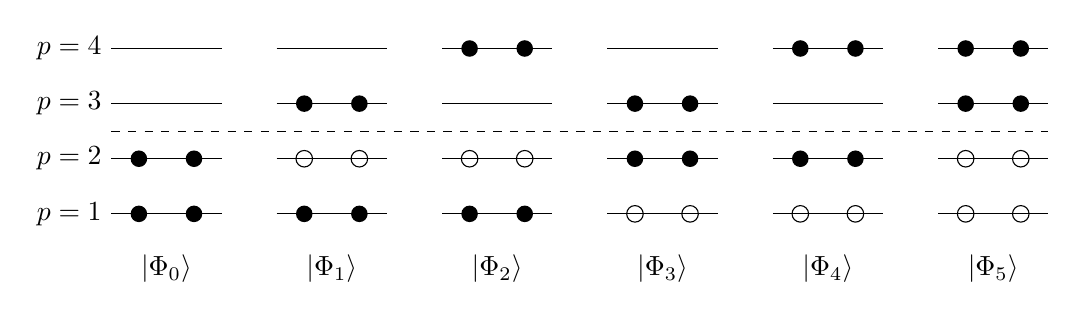
\begin{tikzpicture}[scale=0.7]
    % Draw lines
    \foreach \x in {0,3,6,9,12,15} {
        \foreach \y in {1,2,3,4} {
            \draw (\x, \y) -- (\x+2, \y);
        }
    }
    % Draw additional dashed lines
    \draw[dashed] (0, 2.5) -- (17, 2.5);

    % Labels on the left
    \foreach \y/\label in {1/$p=1$, 2/$p=2$, 3/$p=3$, 4/$p=4$} {
        \node[left] at (0, \y) {\label};
    }

    % Groundstate
    \foreach \x/\y in {0.5/1, 0.5/2, 1.5/1, 1.5/2} {
        \fill (\x, \y) circle (0.15);
    }
    \node at (1, 0) {$|\Phi_0\rangle$};

    % Phi_1
    \foreach \x in {3.5, 4.5} {
        \foreach \y in {1, 3} {
            \fill (\x, \y) circle (0.15);
        }
        \draw (\x, 2) circle (0.15);
    }
    \node at (4, 0) {$|\Phi_1\rangle$};

    % Phi_2
    \foreach \x in {6.5, 7.5} {
        \foreach \y in {1, 4} {
            \fill (\x, \y) circle (0.15);
        }
        \draw (\x, 2) circle (0.15);
    }
    \node at (7, 0) {$|\Phi_2\rangle$};

    % Phi_3
    \foreach \x in {9.5, 10.5} {
        \foreach \y in {2, 3} {
            \fill (\x, \y) circle (0.15);
        }
        \foreach \y in {1} {
            \draw (\x, \y) circle (0.15);
        }
    }
    \node at (10, 0) {$|\Phi_3\rangle$};

    % Phi_4
    \foreach \x in {12.5, 13.5} {
        \foreach \y in {2, 4} {
            \fill (\x, \y) circle (0.15);
        }
        \foreach \y in {1} {
            \draw (\x, \y) circle (0.15);
        }
    }
    \node at (13, 0) {$|\Phi_4\rangle$};

    % Phi_5
    \foreach \x in {15.5, 16.5} {
        \foreach \y in {3, 4} {
            \fill (\x, \y) circle (0.15);
        }
        \foreach \y in {1, 2} {
            \draw (\x, \y) circle (0.15);
        }
    }
    \node at (16, 0) {$|\Phi_5\rangle$};

\end{tikzpicture}

        \caption{
            Schematic representation of the six possible Slater
            determinants for a system with four particles, under the
            constraint of no broken pairs, total spin $S = 0$,
            considering only the four lowest levels $p = 1, 2, 3,
            4$.\label{fig:SDs}
        }
    \end{figure}
\end{frame}

\begin{frame}{Solving the problem}
    In solving the system, one first has to set up the Hamiltonian
    matrix, with elements
    \begin{equation}
        H_{i, j} = \langle \Phi_i \lvert \hat{H} \rvert \Phi_j \rangle,
    \end{equation}
    and then diagonalize the matrix to find the eigenvalues and eigenvectors.
    The ground state energy can then be found as the lowest
    eigenvalue, with the corresponding eigenvector giving the coefficients $C$.

    \bigskip

    FCI is exact, but computationally expensive, as the number of
    configurations grows factorially with the number of energy levels included.
    Approximative methods are therefore required.
\end{frame}

\section{Hartree-Fock}

\begin{frame}{Hartree-Fock theory}
    In Hatree-Fock (HF) theory, we assume that the system can be
    approximated by a single Slater determinant $\Phi$, and we seek
    to find the wavefunctions $\lvert \psi_\alpha \rangle$ that
    minimize the energy
    \begin{equation}
        E_0 = \left\langle \Phi \vert \hat{H} \vert \Phi \right\rangle.
    \end{equation}
    This gives rise to the HF equations
    \begin{equation}\label{eq:HF_equations}
        \hat{h}^\mathrm{HF} \lvert \psi_\alpha \rangle =
        \varepsilon_\alpha \lvert \psi_\alpha \rangle,
    \end{equation}
    where $\hat{h}^\mathrm{HF} = \hat{t} + \hat{u}_{\mathrm{ext}} +
    \hat{u}^\mathrm{HF}$, called the Fock operator, is an effective
    one-body operator.
    Here, $\hat{u}^\mathrm{HF}$ is the mean potential from the other
    particles, of the form
    \begin{equation}\label{eq:HFpotential}
        \langle p \vert \hat{u}^\mathrm{HF} \vert q \rangle =
        \sum_{i} \langle pi \vert V \vert qi \rangle_{AS}.
    \end{equation}
\end{frame}

\begin{frame}{Varying the wave functions}
    As Eq.~\eqref{eq:HFpotential} depends on the eigenfunctions,
    Eq.~\eqref{eq:HF_equations} is nonlinear.
    We therefore solve it iteratively, until convergence is
    reached\footnote{If it converges at all.}.
    Varying the wave functions directly lead to a set of coupled
    integro-differential equations, wherein the integrals need to be
    computed at each iteration.

    \bigskip

    Another, more computationally efficient approach, is to expand
    the wave functions in a basis of known functions, and vary the
    coefficients of the expansion.
    We do this by a unitary transformation to a new basis $p$,
    \begin{equation}
        \psi_p = \sum_{\alpha} C_{p\alpha} \phi_\alpha,
    \end{equation}
    where we now vary the coefficients $C_{p\alpha}$.
\end{frame}

\begin{frame}{The HF equations}
    Varying the coefficients, we find
    \begin{equation}\label{eq:HF_equations_C}
        \sum_{\gamma} h_{\alpha\gamma}^{\mathrm{HF}} C_{p \gamma}
        = \varepsilon_p^{\mathrm{HF}} C_{p \alpha},
    \end{equation}
    where
    \begin{equation}\label{eq:HF_hamiltonian_element}
        h_{\alpha \gamma}^\mathrm{HF}
        = \langle \alpha \vert \hat{h}_0 \vert \gamma \rangle
        + \sum_{\beta\delta} \rho_{\beta\delta} \langle \alpha\beta \vert V \vert \gamma\delta \rangle_{AS}.
    \end{equation}
    Here, $\rho_{\beta\delta}$ is the density matrix, defined as
    $\rho_{\beta\delta} = \sum_{i} \langle \beta \vert i \rangle
    \langle i \vert \delta \rangle = \sum_{i} C_{i\beta} C_{i\delta}^*$.
    Eq.~\eqref{eq:HF_equations_C} is in effect nothing more than an
    eigenvalue problem, and the HF equations are solved by
    diagonalizing the matrix $h^\mathrm{HF}$ repeatedly.
    The efficiency comes from the fact that the integrals in
    Eq.~\eqref{eq:HF_hamiltonian_element} need only be computed once,
    and the density matrix is updated at each iteration from the eigenvectors.
\end{frame}

\section{Many-body pertubation theory}

\begin{frame}{Many-body pertubation theory}
    In many-body pertubation theory (MBPT), we seek to find the
    ground state energy by expanding the wave function in a series of
    pertubations to the Hamiltonian.
    We assume that the exact solution can be written as
    \begin{equation}
        \lvert \Psi_0 \rangle
        = \lvert \Phi_0 \rangle + \sum_{m = 1}^\infty C_m \lvert \Phi_m \rangle,
    \end{equation}
    and that the ground state is dominated by the reference state
    \begin{equation}
        \hat{H}_0 \lvert \Phi_0 \rangle = W_0 \lvert \Phi_0 \rangle.
    \end{equation}
\end{frame}

\begin{frame}{Correlation energy}
    The Schrödinger equation is then
    \begin{equation}
        \hat{H} \lvert \Psi_0 \rangle = E \lvert \Psi_0 \rangle,
    \end{equation}
    which gives
    \begin{equation}
        \left\langle \Phi_0 \vert \hat{H} \vert \Psi_0 \right\rangle = E.
    \end{equation}
    % \begin{align}
    %     \hat{H} \lvert \Psi_0 \rangle = E \lvert \Psi_0 \rangle,
    %     \quad \text{which gives} \quad
    %     \left\langle \Phi_0 \vert \hat{H} \vert \Psi_0 \right\rangle = E.
    % \end{align}
    Combining this with
    \begin{equation}
        \left\langle \Psi_0 \vert \hat{H}_0 \vert \Phi_0 \right\rangle = W_0,
    \end{equation}
    and using the fact that $\hat{H}, \hat{H}_0$ are Hermitian, we find
    \begin{equation}\label{eq:corr_energy_original}
        \left\langle \Phi_0 \vert \hat{H}_I \vert \Psi_0 \right\rangle
        = E - W_0
        = \Delta E,
    \end{equation}
    where $\Delta E$ is the correlation energy.
\end{frame}

\begin{frame}{Perturbed expression}
    Introducing the energy variable $\omega$, we can derive
    \begin{equation}\label{eq:corr_energy}
        \Delta E = \sum_{i = 0}^\infty \Big\langle \Phi_0 \big\vert \hat{H}_I \left\{
            \frac{\hat{Q}}{\omega - \hat{H}_0} \left( \omega - E + \hat{H}_I \right)
        \right\}^{i} \big\lvert \Phi_0 \Big\rangle.
    \end{equation}
    This is in reality nothing more than a rewrite of Eq.~\eqref{eq:corr_energy_original}, but serves as a starting point for the pertubation expansion.
    It contains the unknown energy $E$, as well as the variable $\omega$, and hence we need further assumptions to solve it.
\end{frame}

\subsection{Brillouin-Wigner}

\begin{frame}{Brillouin-Wigner pertubation theory}
    In Brillouin-Wigner pertubation theory (BWPT), we set $\omega = E$ in Eq.~\eqref{eq:corr_energy}, and we find
    \begin{equation}
        \begin{split}
            \Delta E &= \sum_{i = 0}^\infty \Big\langle \Phi_0 \big\vert \hat{H}_I \left\{
                \frac{\hat{Q}}{E - \hat{H}_0} \hat{H}_I
            \right\}^{i} \big\lvert \Phi_0 \Big\rangle \\
            &= \Big\langle \Phi_0 \vert \left( \hat{H}_I + \hat{H}_I \frac{\hat{Q}}{E - \hat{H}_0} \hat{H}_I + \hat{H}_I \frac{\hat{Q}}{E - \hat{H}_0} \hat{H}_I \frac{\hat{Q}}{E - \hat{H}_0} \hat{H}_I + \ldots \right) \big\lvert \Phi_0 \Big\rangle.
        \end{split}
    \end{equation}
    The equations then become rather simple, as compared with Eq.~\eqref{eq:corr_energy}, with the exception on the unknown energy $E$.
    It can however be solved iteratively, for an initial guess of $E$.
\end{frame}

\subsection{Rayleigh-Schrödinger}

\begin{frame}{Rayleigh-Schrödinger pertubation theory}
    In Rayleigh-Schrödinger pertubation theory (RSPT), we set $\omega = W_0$ in Eq.~\eqref{eq:corr_energy}, and we find
    \begin{equation}
        \begin{split}
            \Delta E &= \sum_{i = 0}^\infty \Big\langle \Phi_0 \big\vert \hat{H}_I \left\{
                \frac{\hat{Q}}{W_0 - \hat{H}_0} \left( W_0 - E + \hat{H}_I \right)
            \right\}^{i} \big\lvert \Phi_0 \Big\rangle \\
            &= \sum_{i = 0}^\infty \Big\langle \Phi_0 \big\vert \hat{H}_I \left\{
                \frac{\hat{Q}}{W_0 - \hat{H}_0} \left( \hat{H}_I - \Delta E \right)
            \right\}^{i} \big\lvert \Phi_0 \Big\rangle.
        \end{split}
    \end{equation}
    As $\hat{Q} \Delta E \vert \Phi_0 \rangle = 0$, we can write
    \begin{equation}\label{eq:RSPT}
        \Delta E = \Big\langle \Phi_0 \big\vert
        \hat{H}_I
        + \hat{H}_I \frac{\hat{Q}}{W_0 - \hat{H}_0} \hat{H}_I
        + \hat{H}_I \frac{\hat{Q}}{W_0 - \hat{H}_0} \left( \hat{H}_I - \Delta E \right) \frac{\hat{Q}}{W_0 - \hat{H}_0} \hat{H}_I
        + \ldots
        \big\vert \Phi_0 \Big\rangle.
    \end{equation}
\end{frame}

\begin{frame}{Order by order contributions}
    Eq.~\eqref{eq:RSPT} allows us to define the recursive formula
    \begin{equation}
        \Delta E = \sum_{i = 1}^\infty \Delta E^{(i)},
    \end{equation}
    where the first few terms are, writing $\langle \hat{A} \rangle = \langle \Phi_0 \vert \hat{A} \vert \Phi_0 \rangle$,
    \begin{align}
        \Delta E^{(1)} &= \Big\langle \hat{H}_I \Big\rangle \\
        \Delta E^{(2)} &= \Big\langle \hat{H}_I \frac{\hat{Q}}{W_0 - \hat{H}_0} \hat{H}_I \Big\rangle \\
        \Delta E^{(3)} &=
        \Big\langle
        \hat{H}_I \frac{\hat{Q}}{W_0 - \hat{H}_0}
        \hat{H}_I \frac{\hat{Q}}{W_0 - \hat{H}_0}
        \hat{H}_I
        \Big\rangle
        - \Big\langle
        \hat{H}_I \frac{\hat{Q}}{W_0 - \hat{H}_0}
        \Big\langle \hat{H}_I \Big\rangle
        \frac{\hat{Q}}{W_0 - \hat{H}_0} \hat{H}_I
        \Big\rangle.
    \end{align}
\end{frame}

\begin{frame}{Order by order contributions}
    With the previous formula, we can find the correlation energy up to a given order of contributions.
    This method is however not without its drawbacks.
    For one, there is no guarantee that the series will converge, and the method is not variational.
    This entails that we will not necessarily get an improved estimate from including more terms in the series.
\end{frame}

\section{Coupled-Cluster theory}

\begin{frame}{Coupled-Cluster theory}
    In coupled-cluster (CC) theory, we seek to write the wave function as
    \begin{equation}
        \lvert \Psi_0 \rangle = e^{\hat{T}} \lvert \Phi_0 \rangle,
    \end{equation}
    where $\hat{T}$ is the cluster operator, defined as
    \begin{equation}
        \hat{T} = \hat{T}_1 + \hat{T}_2 + \hat{T}_3 + \ldots,
    \end{equation}
    with $\hat{T}_n$ being the $n$-body cluster operator.
    The first two such operators are
    \begin{equation}
        \hat{T}_1 = \frac{1}{(1!)^2}\sum_{ai} t_i^a a_a^\dagger a_i,
        \quad \text{and} \quad
        \hat{T}_2 = \frac{1}{(2!)^2} \sum_{abij} t_{ij}^{ab} a_a^\dagger a_b^\dagger a_j a_i.
    \end{equation}
    With this, we also define the similarity transformed Hamiltonian $\overline{H_N} = e^{-\hat{T}} \hat{H} e^{\hat{T}}$.
\end{frame}

\begin{frame}{Determining the cluster amplitudes}
    We determine the cluster amplitudes $t_{i_1 \ldots i_n}^{a_1 \ldots a_n}$ by solving the equations
    \begin{equation}
        \Big\langle \Phi_{i_1 \ldots i_n}^{a_1 \ldots a_n} \vert \overline{H_N} \vert \Phi_0 \Big\rangle = 0,
    \end{equation}
    which is derived from the equations
    \begin{equation}
        \Big\langle \Phi_{i_1 \ldots i_n}^{a_1 \ldots a_n} \vert \hat{H}  e^{\hat{T}} \vert \Phi_0 \Big\rangle = E_0 \Big\langle \Phi_{i_1 \ldots i_n}^{a_1 \ldots a_n} \vert e^{\hat{T}} \vert \Phi_0 \Big\rangle.
    \end{equation}
    If we were to solve this exactly without truncations, i.e.\ by including up to $np$--$nh$ excitations, we would have the same complexity as FCI. % chktex 13
    We therefore need to truncate the series, and the most common truncation is at CCSD, where we include up to $2p$--$2h$ excitations.
\end{frame}

\begin{frame}{Truncated Couple-Cluster}
    In order to make the method computationally feasible, we truncate the series at some level.
    By doing this, the method is non-variational.

    \bigskip

    We solve the equations iteratively, and in this case we need an initial guess for the cluster amplitudes.
    A common choice in CCD is then to use the first order wave operator from MPBT, setting
    \begin{equation}
        (t_{ij}^{ab})^{(0)} = \frac{
            \langle ab \vert V \vert ij \rangle
        }{
            \varepsilon_i + \varepsilon_j - \varepsilon_a - \varepsilon_b
        }.
    \end{equation}
\end{frame}

\begin{frame}{CCD results for the pairing model}
    \begin{columns}
        \begin{column}{.49\textwidth}
            Returning to the pairing model, we have the ground state energy difference for the CCD method, as a function of the interaction strength $g$.
        \end{column}

        \begin{column}{.49\textwidth}
            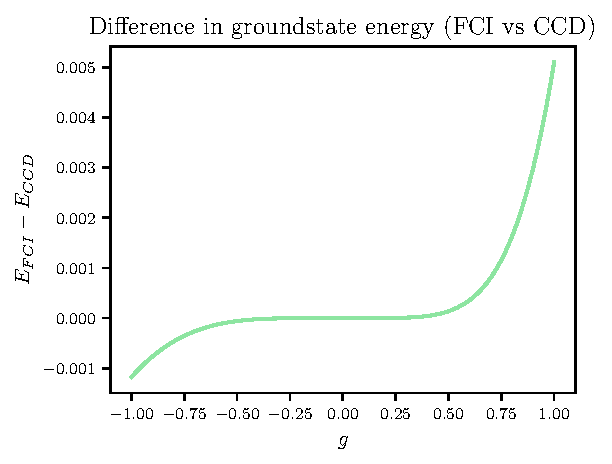
\includegraphics[width=\textwidth]{../midterm2/figures/ccd_groundstate_energy_diff.pdf}
        \end{column}
    \end{columns}
\end{frame}

\uiofullpageimage{../midterm2/figures/absolute_differences.pdf}

\appendix
\section{Derivation of the HF equations}

\begin{frame}{Derivation of the HF equations}
    In the original basis $\alpha$ we have the energy functional
    \begin{equation}
        E[\Phi]
        = \left\langle \Phi \vert \hat{H} \vert \Phi \right\rangle
        = \sum_{\alpha} \langle \alpha \vert \hat{h}_0 \vert \alpha \rangle
        + \frac{1}{2} \sum_{\alpha\beta} \langle \alpha\beta \vert V
        \vert \alpha \beta \rangle_{AS}.
    \end{equation}
    By way of varying the coefficients, the HF equations are found by
    introducing the new basis $p$ defined by the unitary transformation
    \begin{equation}
        \psi_p = \sum_{\alpha} C_{p\alpha} \phi_\alpha,
    \end{equation}
    and minimizing the energy functional
    \begin{equation}\label{eq:PhiHF}
        E[\Phi^\mathrm{HF}]
        = \left\langle \Phi^\mathrm{HF} \vert \hat{H} \vert
        \Phi^\mathrm{HF} \right\rangle
        = \sum_{i} \langle i \vert \hat{h}_0 \vert i \rangle +
        \frac{1}{2} \sum_{ij} \langle ij \vert V \vert ij \rangle_{AS}
    \end{equation}
    with respect to the coefficients $C_{p\alpha}$.
\end{frame}

\begin{frame}{Introducing Lagrange multipliers}
    Defining the functional in Eq.~\eqref{eq:PhiHF} as a functional
    of the coefficients $C_{p\alpha}$, we have
    \begin{equation}%\label{eq:E0}
        E_0[C]
        = \sum_{i} \sum_{\alpha\beta} {
            C_{i \alpha}^*
            C_{i \beta}
            \langle \alpha \vert \hat{h}_0 \vert \beta \rangle
        }
        + \frac{1}{2} \sum_{ij} \sum_{\alpha\beta\gamma\delta} {
            C_{i \alpha}^*
            C_{j \beta}^*
            C_{i \gamma}
            C_{j \delta}
            \langle \alpha\beta \vert V \vert \gamma\delta \rangle_{AS}
        }.
    \end{equation}
    As we have orthonormal basis functions, we have
    \begin{equation}
        \langle i \vert j \rangle
        = \delta_{ij}
        = \sum_{\alpha\beta} C_{i\alpha}^* C_{i\beta}
        \langle \alpha \vert \beta \rangle
        = \sum_{\alpha} C_{i\alpha}^* C_{i\alpha},
    \end{equation}
    so we introduce the functional
    \begin{equation}
        F[C] = E_0[C] - \sum_{i} \lambda_i \sum_{\alpha}
        C_{i\alpha}^* C_{i\alpha},
    \end{equation}
    where $\lambda_i$ are the Lagrange multipliers enforcing orthonormality.
\end{frame}

\begin{frame}{Minimizing $F$}
    Minimizing $F$ with respect to $C^*_{i\alpha}$, we wish to solve
    \begin{equation}
        \frac{\diff F}{\diff C^*_{i\alpha}}[C] = \frac{\diff}{\diff
        C_{i \alpha}^*} \left[ E_0[C] - \sum_j \lambda_j
        \sum_{\alpha} C_{j \alpha}^* C_{j \alpha} \right] = 0.
    \end{equation}

    Term by term we have
    \begin{align}
        \frac{\diff}{\diff C_{i \alpha}^*} \sum_{i}
        \sum_{\alpha\beta} C_{i \alpha}^* C_{i \beta}
        \langle \alpha \vert \hat{h}_0 \vert \beta \rangle
        &= \sum_{\beta} C_{i \beta}
        \langle \alpha \vert \hat{h}_0 \vert \beta \rangle \\
        \frac{\diff}{\diff C_{i \alpha}^*}
        \frac{1}{2} \sum_{ij} \sum_{\alpha\beta\gamma\delta} C_{i
        \alpha}^* C_{j \beta}^* C_{i \gamma} C_{j \delta}
        \langle \alpha\beta \vert V \vert \gamma\delta \rangle_{AS}
        &= \sum_j \sum_{\beta\gamma\delta} C_{j \beta}^* C_{i \gamma}
        C_{j \delta} \langle \alpha\beta \vert V \vert \gamma\delta
        \rangle_{AS},
    \end{align}
\end{frame}

\begin{frame}{Minimizing $F$, cont.}
    and finally
    \begin{equation}
        \frac{\diff}{\diff C_{i \alpha}^*} \sum_{i} \lambda_i
        \sum_{\alpha} C_{i \alpha}^* C_{i \alpha} = \lambda_i C_{i \alpha}.
    \end{equation}

    \bigskip

    Combining these terms, we have
    \begin{equation}
        \sum_{\beta} C_{i \beta}
        \langle \alpha \vert \hat{h}_0 \vert \beta \rangle
        + \sum_j \sum_{\beta\gamma\delta} C_{j \beta}^* C_{i \gamma}
        C_{j \delta} \langle \alpha\beta \vert V \vert \gamma\delta \rangle_{AS}
        - \lambda_i C_{i \alpha} = 0.
    \end{equation}

    Recognizing $\lambda_i$ as the eigenvalues
    $\varepsilon_i^\mathrm{HF}$, we can write this as
    \begin{equation}
        \sum_{\gamma} \left[
            \langle \alpha \vert \hat{h}_0 \vert \gamma \rangle
            + \sum_j \sum_{\beta\delta} C_{j \beta}^*  C_{j \delta}
            \langle \alpha\beta \vert V \vert \gamma\delta \rangle_{AS}
        \right] C_{p \gamma}
        = \varepsilon_p^\mathrm{HF} C_{p \alpha}.
    \end{equation}
\end{frame}

\begin{frame}{Hartree-Fock equations found}
    This finally results in the HF equations
    \begin{equation}
        \sum_{\gamma} h_{\alpha\gamma}^\mathrm{HF} C_{p \gamma} =
        \varepsilon_p^\mathrm{HF} C_{p \alpha}.
    \end{equation}
\end{frame}

\section{Derivation of MBPT}
\begin{frame}{Derivation of many-body pertubation expansion}
    We have
    \begin{align}
        \hat{H} \lvert \Psi_0 \rangle &= E \lvert \Psi_0 \rangle \\
        \left( \hat{H}_0 + \hat{H}_I \right) \lvert \Psi_0 \rangle &= E \lvert \Psi_0 \rangle \\
        -\hat{H}_0 \lvert \Psi_0 \rangle &= \left( - E + \hat{H}_I \right) \lvert \Psi_0 \rangle \\
        \left( \omega - \hat{H}_0 \right) \lvert \Psi_0 \rangle &= \left(\omega - E + \hat{H}_I \right) \lvert \Psi_0 \rangle,
    \end{align}
    where $\omega$ is an energy variable dependent on the expansion method.
    Assuming the resolvent of $\left( \omega - \hat{H}_0 \right)$ exists, we can then rewrite the Schrödinger equation as
    \begin{equation}
        \lvert \Psi_0 \rangle = \frac{1}{\omega - \hat{H}_0} \left( \omega - E + \hat{H}_I \right) \lvert \Psi_0 \rangle.
    \end{equation}
\end{frame}

\begin{frame}{Combining with projection operators}
    With the projection operators
    \begin{equation}
        \hat{P} = \lvert \Phi_0 \rangle \langle \Phi_0 \rvert
        \quad \text{and} \quad
        \hat{Q} = \sum_{m = 1}^\infty \lvert \Phi_m \rangle \langle \Phi_m \rvert,
    \end{equation}
    we can then write
    \begin{equation}
        \begin{split}
            \lvert \Psi_0 \rangle
            &= \left( \hat{P} + \hat{Q} \right) \lvert \Psi_0 \rangle
            = \vert \Phi_0 \rangle + \hat{Q} \lvert \Psi_0 \rangle \\
            &= \vert \Phi_0 \rangle + \frac{\hat{Q}}{\omega - \hat{H}_0} \left( \omega - E + \hat{H}_I \right) \lvert \Psi_0 \rangle.
        \end{split}
    \end{equation}
    Solving this in an iterative fashion, with an initial guess for $\lvert \Psi_0 \rangle = \lvert \Phi_0 \rangle$, we have
    \begin{equation}
        \vert \Psi_0 \rangle = \sum_{i = 0}^\infty \left\{
            \frac{\hat{Q}}{\omega - \hat{H}_0} \left( \omega - E + \hat{H}_I \right)
        \right\}^{i} \lvert \Phi_0 \rangle.
    \end{equation}
\end{frame}

% TODO: Add something about Pauli Exclusion Principle in Appendix

\end{document}
